\documentclass[12pt,a4paper]{article}
\usepackage[UTF8]{ctex}
\usepackage{amsmath,amssymb}
\usepackage{xcolor}
\usepackage{hyperref}
\usepackage{geometry}
\usepackage{graphicx}
\geometry{margin=2.5cm}

\title{Rejection Sampling / 拒绝采样}
\author{QuoNic}
\date{}

\begin{document}
\maketitle

\begin{center}
\textbf{Algorithms / 算法} | 难度：中级 | 预计时间：10 分钟
\end{center}

\tableofcontents
\newpage

\section{为什么需要？}

拒绝采样用于从复杂分布中采样。

\subsection{经典局限}
\begin{itemize}
  \item 经典拒绝采样效率低
  \item 对于复杂分布，拒绝率高
\end{itemize}

\subsection{量子优势}
\begin{itemize}
  \item 量子拒绝采样可以利用量子叠加
  \item 提高采样效率
  \item 可以处理更复杂的分布
\end{itemize}

\subsection{实际应用}
\begin{itemize}
  \item 量子采样
  \item 量子模拟
  \item 量子机器学习
\end{itemize}

\section{快速上手}

\begin{verbatim}
from quonic.algorithms import rejection_sampling

# 拒绝采样
result = rejection_sampling(target='11', n_qubits=2)
print(f'Samples: {result.samples}')
\end{verbatim}

\textbf{预期输出}：
\begin{verbatim}
Samples: ['11', '11', '11', ...]
\end{verbatim}

\section{原理详解}

\subsection{电路图}

\begin{center}
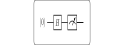
\includegraphics[width=0.6\textwidth]{../../images/rejection_sampling_circuit.svg}
\end{center}

\subsection{数学推导}

拒绝采样：
\begin{equation}
P(\text{accept}) = \frac{f(x)}{M \cdot g(x)}
\end{equation}

其中 $f(x)$ 是目标分布，$g(x)$ 是提议分布，$M$ 是常数。

\subsection{几何解释}

拒绝采样在 Bloch 球上从提议分布中采样，然后根据接受概率决定是否接受。

\section{代码详解}

\begin{verbatim}
from quonic.algorithms import rejection_sampling

# rejection_sampling(target, n_qubits, n_samples)
# target: 目标态
# n_qubits: 量子比特数
# n_samples: 采样数

result = rejection_sampling(
    target='11',
    n_qubits=2,
    n_samples=100
)

# result.samples: 采样结果
# result.acceptance_rate: 接受率
print(f'Samples: {result.samples}')
\end{verbatim}

\section{进阶用法}

\subsection{场景 1：不同目标态}

\begin{verbatim}
from quonic.algorithms import rejection_sampling

# 不同目标态
r1 = rejection_sampling(target='00', n_qubits=2)
r2 = rejection_sampling(target='11', n_qubits=2)
r3 = rejection_sampling(target='101', n_qubits=3)
\end{verbatim}

\section{适用场景}

\subsection{量子采样}

拒绝采样用于从复杂量子分布中采样。例如，从量子玻尔兹曼机中采样。

\subsection{量子模拟}

拒绝采样用于量子模拟中的采样。例如，从量子态中采样。

\section{常见问题}

\subsection{拒绝采样和直接采样有什么区别？}

拒绝采样从提议分布中采样，然后根据接受概率决定是否接受。直接采样从目标分布中直接采样。

\subsection{拒绝采样的效率如何？}

拒绝采样的效率取决于接受率。接受率越高，效率越高。

\section{学习路径}

\subsection{前置知识}
\begin{itemize}
  \item 量子采样
  \item 概率分布
  \item 量子测量
\end{itemize}

\subsection{继续学习}
\begin{itemize}
  \item 量子采样
  \item 量子模拟
  \item 量子机器学习
\end{itemize}

\section{完整示例代码}

\subsection{示例 1：基本拒绝采样}

\begin{verbatim}
from quonic.algorithms import rejection_sampling

result = rejection_sampling(target='11', n_qubits=2)
print(f'Samples: {result.samples}')
\end{verbatim}

\section{下载}

\begin{itemize}
  \item [rejection\_sampling.py](https://github.com/ChrisLee0721/QuoNic/blob/main/examples/rejection_sampling/rejection_sampling.py)
\end{itemize}

\end{document}
